\chapter{Programming project description}
\label{chap:project}
\section{Introduction}

Programming project of this thesis is a set of command line programs, collectively
called \emph{Karstgen}, that take
the description of karst cave fracture net and generate polygon mesh in
simple and popular Wavefront OBJ textual file format\footnote{\url{http://www.martinreddy.net/gfx/3d/OBJ.spec}}.

Models created this way may be opened in 3D editing program for further editing
and examination.

Karstgen can also create models for \emph{Vorticity} game engine that was created
by the author together with mr Michał Siejak for graphics related courses\footnote{Computer
  Graphics and Visualiation, summer semester 2009/2009 and Group Project, summer
semester 2009/2010} during licenciate studies at Adam Mickiewicz University \todo{check form}in
Poznań.

\section{Architecture}

Karstgen was created with Unix Philosophy in mind \parencite{raymond2003art}.
It is made of two programs named \emph{blobber} and \emph{mcblob} that have
clearly defined reposinsibilities and communicate through simple textual data
format.  Both programs may take input either from files or from standard input
so they can be piped together with shell pipes. Data flow of karstgen is
presented in \autoref{fig:karstgenflow}.
\begin{figure}[ht]
  \begin{center}
    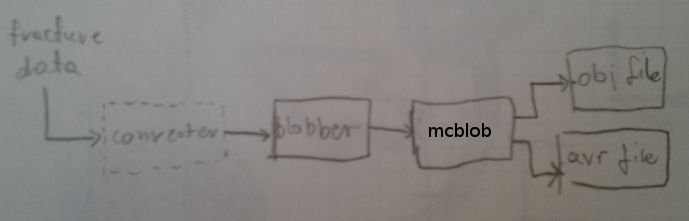
\includegraphics[width=\textwidth]{chapters/project/karstgenflow.jpg}
  \end{center}
  \caption{Data flow of karstgen program. Converter part is required when fracture
  net description is other than expected by blobber.}
  \label{fig:karstgenflow}
\end{figure}
\todo{replace \autoref{fig:karstgenflow} with TikZ graphics}

\subsection{Blobber}
Blobber takes description of a fracture net in a simple textual format and
generates list of metaballs (see \autoref{sub:metaballs}). It can
optionally tilt positions and sizes of metaballs in random but adjustable manner
for more natural--looking results. Blobber also controls quality of the final
geometry. For information about runtime parameters invoke:
\begin{verbatim}
./blobber --help
\end{verbatim}

\subsection{Mcblob}
Output generated by blobber is consumed by program named \emph{mcblob}\footnote{Marching
Cubes from blobs} which is general purpose tool that may be used to
generate geometry from a list of metaballs in 3D space.

\section{Implementation}
\subsection{Metaballs}
Implementation heavily relies on rendering with metaballs. Metaball in 3D space
is a scalar function in the form:
\begin{equation}
  f(x,y,z)=Te^{\frac{B}{R^2}r^2 - B}
  \label{eq:metaball}
\end{equation}
where $r$ is distance from point $(x,y,z)$ to the center of the metaball, $B$ is
,,blobiness'' factor that controls tendency to ,,melt'' with other metaballs, $T$
is isovalue that will be used for rendering and $R$ is the radius of the
metaball if it was isolated from other blobs. This equation is basically a
Gaussian bump centerd at the center of the metaball.

If more than one metaball is present in the scene, density function (see Definition
\autoref{def:density function})
is in the form:
\begin{equation}
  d(x,y,z) = \sum_{i=0}^{n} f_i(x,y,z)
  \label{eq:metaballdensity}
\end{equation}
where $n$ is the total number of metaballs in the scene and $f_i$ is function~\ref{eq:metaball}
of the $i$-th metaball.

Metaballs were discovered by Jim Blinn when he was working on visualisation of
molecular structures \parencite{Blinn:1982:GAS:357306.357310}. Density function 
was derieved from equation defining density of electron field of hydrogen atom
as used in quantum mechanics.

This ,,melting'' property visible when metaballs are close to each other gives
somewhat ,,organic'' look and feel of structures generated with them
(see \autoref{fig:metaballs}).
\label{sub:metaballs}
\begin{figure}[htb]
  \begin{center}
    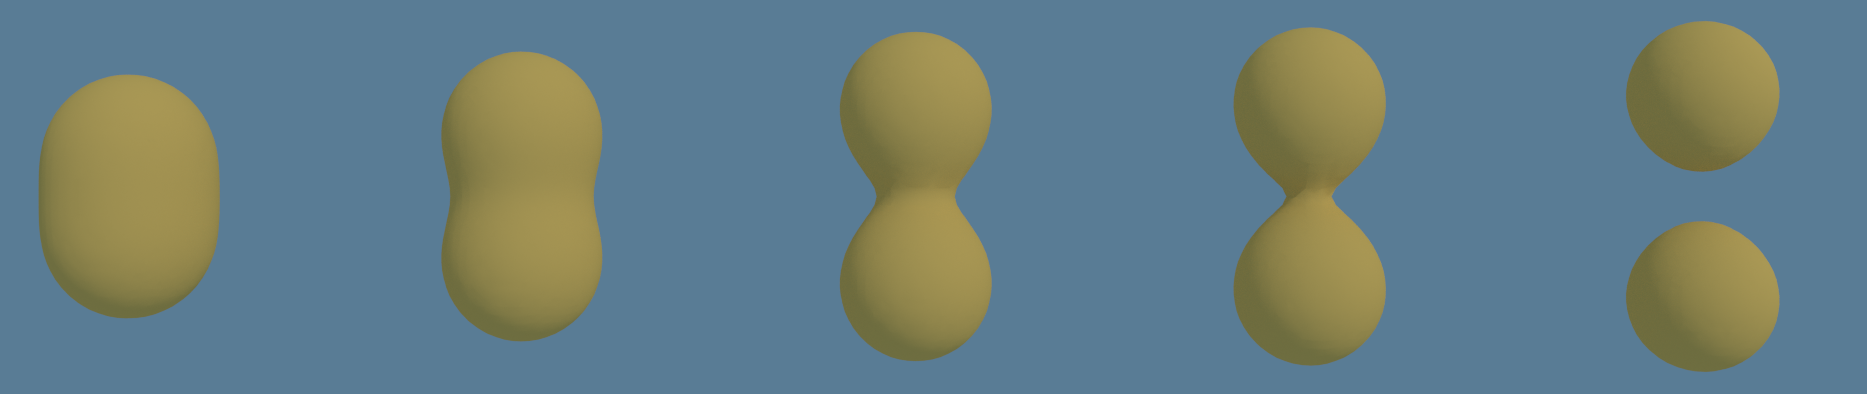
\includegraphics[width=\textwidth]{chapters/project/metaballs.png}
  \end{center}
  \caption{Two metaballs at various distances showing how they are ,,melitng''
    together when getting closer to each other. Geometry was generated with
    \emph{mcblob} program and final image was rendered with Blender 2.68 with
    Cycles renderer. Input file for mcblob that generates this is included with the thesis
      in \texttt{fig\_metaballs.in} file in kartsgen examples.
  }
  \label{fig:metaballs}
\end{figure}


\subsection{Overview}
Both blobber and mcblob are implemented in C++ language with latest C++11
version of the standard. Build system used to compile the code is \emph{CMake}\footnote{Cross--platform make}
-- meta build system that can generate native projects for various IDEs\footnote{Integrated Development Environment}
andactual build systems. Executables use \emph{Boost Program Options} library
for parsing command line arguments and providing help.

Karstgen uses unit testing framework \emph{Google~Test}\footnote{\url{http://code.google.com/p/googletest/}}.
Documentation is automatically generated from sources with Doxygen
tool.


\subsection{Blobber}

For vector data structuers blobber uses \emph{GLM}\footnote{\url{http://glm.g-truc.net/0.9.4/index.html}}
-- a mathematical library that resembles GLSL\footnote{OpenGL Shading Language}.

It reads information about diameters of fractures in fractures network
and places blobs along these fractures with diameters roughly the same as of
these fractures.

Blobber works on data structure named \texttt{DataPoint}:

\begin{lstlisting}
struct DataPoint
{
  	int x, y, z;
	float midDiam;
	std::vector<float> xData;
	std::vector<float> yData;
	std::vector<float> zData;
};
\end{lstlisting}

This structure can describe three fractures originating in index $(x,y,z)$ in
the fracture net and going along each axe in ascending direction. Each fracture
is described as a vector of uniformly distributed diameters. If there is only
one diameter in a vector it is assumed that the fraction it represens has the
same diameter along its whole length. When no diameters are present in some
vector, it is assumed that there is no fracture in this direction.
Additional field \texttt{midDiam} is a diameter of blob that should be placed in
the intersection of the three fractures.

\begin{figure}[hb]
  \begin{center}
    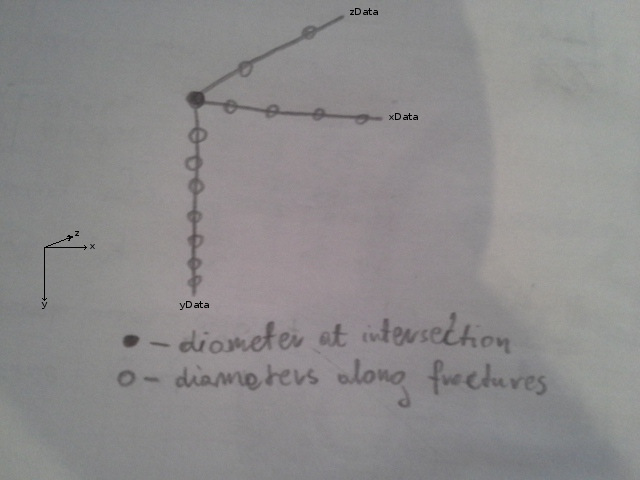
\includegraphics[width=0.7\textwidth]{chapters/project/datapoint.jpg}
  \end{center}
  \caption{Graphical representation of \texttt{dataPoint} -- a basic structure that
blobber works on}
  \label{fig:datapoint}
\end{figure}

Data points are packed into a structure representing whole fracture network
called \texttt{FractureNet}:
\begin{lstlisting}[label={lst:fracturenet},escapeinside={@}{@}]
struct FractureNet
{
	//size of net in number of dataPoints
	int x; int y; int z;
	
	//length of single fracture in each direction
	float xLen; float yLen; float zLen;
	
	std::map<std::tuple<int, int, int>, DataPoint> dataPoints;
};
\end{lstlisting}

Since fracture net is usually quite sparse, dictionary structure\footnote{\texttt{std::map} from C++'s Standard Template Library}
is used to store data points instead of array or vector. Keys in this dictionary
are tuples containing 3D index in a fracture net. This way, given one data point
it is easy to find its neighbours.

\subsubsection{Placement of blobs}

Blobber works on one data point at a time through \texttt{blobs\-From\-Data\-Point()}
function. First, one point is placed in the intersection of the axes with
diameter equal to \texttt{mid\-Point\-Diam}. Then, vector for each non--empty
axe is processed by \texttt{blobsOnVector()} function. Besides the vector of
diameters, this function takes \texttt{midPointDiam} of the data point, and optionally
\texttt{nextDpMidDiam} which is \texttt{midPointDiam} of the next data point
along this axis if such data point exists. Fast lookup of next data point
is possible thanks to dictionary storage of data points. If there is no neighbour data
point at the end of the axis, \texttt{nextDpMidDiam} is considered to be 0.\todo{test if this makes sense}

\begin{figure}[htb]
  \begin{center}
    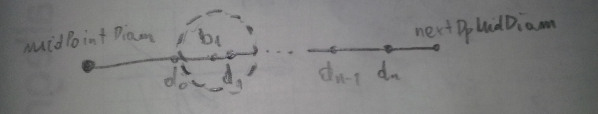
\includegraphics[width=\textwidth]{chapters/project/placement.jpg}
  \end{center}
  \caption{Blobs are placed along fracture defined as set of diameters
    $(d_0,d_1,\cdots,d_{n-1})$. In this example diameter of blob $b_1$ will be a
    linear interpolation of diameters $d_0$ and $d_1$ proportional to distance
    from these diameters.}
  \label{fig:placement}
\end{figure}

Function \texttt{blobsOnVector()} places blobs on the fracture line until
it's fully covered. Diameters of blobs are determined in a way described
in \autoref{fig:placement}.

Format of the input to blobber is described in generated documentation:
\begin{lstlisting}[language=bash,numbers=none]
\doc\blobber\html\index.html
\end{lstlisting}

Output format is the same as input format of mcblob program and is described in
its help:
\begin{lstlisting}[language=bash,numbers=none]
./mcblob --help
\end{lstlisting}

\subsection{Mcblob}
\label{sub:mcblob}

Mcblob uses OpenCL (\autoref{chap:cl}) to calculate density function from
list of blobs provided in input, generates polygon mesh of isosurface
definded by this function using Marching Cubes algorithm (\autoref{chap:marchingcubes})
accelerated with OpenCL and saves results to file in one of two formats.

Bounds of 3D space within which geometry will be generated is defined in input.
It's divided into blocks which are worked on one at a time. For each block,
density function is calculated from blobs, followed by generating geometry.

Finally, when geometry from all blocks is calculated, mcblob writes output to
disk in one of two supported formats.

\subsubsection{Calculating density function}

Each block of voxels is kept by mcblob in a class called \texttt{Grid}. It
contains values of density function on the vertices of the cubes in a block.
These values are stored as one--dimensional array, that is transferable between host and
device memory. If number of voxels on $x$, $y$ and $z$ axes is $v_x$, $v_y$
and $v_z$ respectively, \texttt{Grid} will store 1D array
of \texttt{float4} values $(v_x+1)\times(v_y+1)\times(v_z+1)$ elements long.

\begin{figure}[tb]
  \begin{center}
    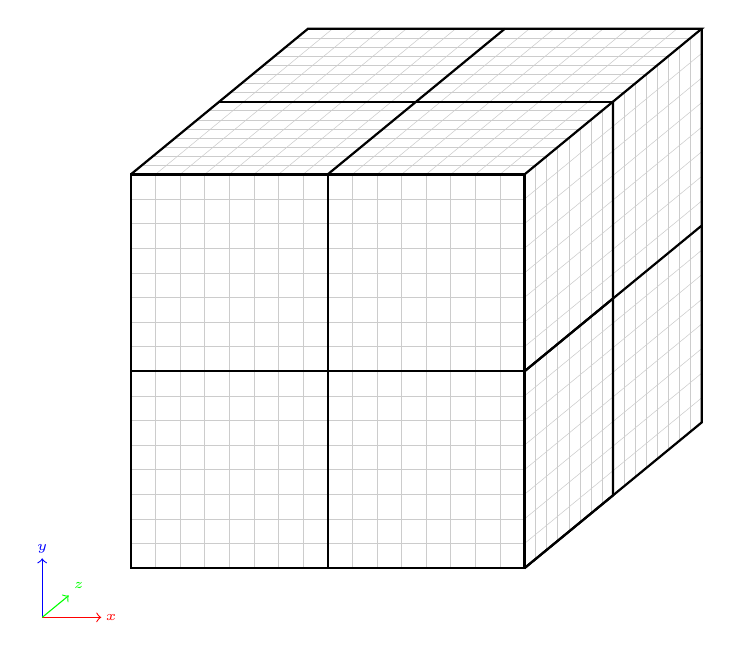
\begin{tikzpicture}[z={(-0.45cm,-0.37cm)}, scale=2.5]

\tikzstyle{inner} = [gray!40!white,very thin]
%front face vertical
\foreach \x in {1,2,3,4,5,6,7,9,10,11,12,13,14,15}
  \draw[inner] (\x/8,0) -- (\x/8,2);
%front face horizontal
\foreach \x in {1,2,3,4,5,6,7,9,10,11,12,13,14,15}
  \draw[inner] (0,\x/8) -- (2,\x/8);

%rigt face vertical
\foreach \x in {1,2,3,4,5,6,7,9,10,11,12,13,14,15}
  \draw[inner] (2,0,-\x/8) -- (2,2,-\x/8);
%rigth face horizontal
\foreach \x in {1,2,3,4,5,6,7,9,10,11,12,13,14,15}
  \draw[inner] (2,\x/8,0) -- (2,\x/8,-2);

%top face front to back
\foreach \x in {1,2,3,4,5,6,7,9,10,11,12,13,14,15}
  \draw[inner] (\x/8,2,0) -- (\x/8,2,-2);
%top face left to rigth
\foreach \x in {1,2,3,4,5,6,7,9,10,11,12,13,14,15}
  \draw[inner] (0,2,-\x/8) -- (2,2,-\x/8);


\draw[thick] (0,0) rectangle (1,1);
\draw[thick] (1,0) rectangle (2,1);
\draw[thick] (0,1) rectangle (1,2);
\draw[thick] (1,1) rectangle (2,2);

\draw[thick] (2,1) -- (2,1,-1) -- (2,2,-1);
\draw[thick] (2,1) -- (2,1,-2) -- (2,2,-2);
\draw[thick] (2,0) -- (2,0,-1) -- (2,1,-1);
\draw[thick] (2,0) -- (2,0,-2) -- (2,1,-2);

\draw[thick] (1,2) -- (1,2,-2);
\draw[thick] (0,2,-1) -- (2,2,-1);

\draw[thick] (0,2) -- (0,2,-2) -- (2,2,-2) -- (2,2);

\draw[red,->] (-0.45,-0.25) -> (-0.15,-0.25) ;
\draw[red] (-0.1, -0.25) node[font=\tiny] {$x$};

\draw[blue,->] (-0.45,-0.25) -> (-0.45, 0.05);
\draw[blue] (-0.45, 0.1) node[font=\tiny] {$y$};


\draw[green,->] (-0.45,-0.25) -> (-0.45, -0.25, -0.3);
\draw[green] (-0.40, -0.20, -0.3) node[font=\tiny] {$z$};

\end{tikzpicture}
  \end{center}
  \caption{In this configuration, domain is divided into $2\times2\times2=8$
  grids, and each one of them consists of $8\times8\times8=512$ voxels totalling
 $512\times8=4096$ voxels.}
  \label{fig:grid}
\end{figure}

Four floats are kept for each vertex instead of one to facilitate computation of
normal vectors. In case of \texttt{Grid} components $x$, $y$ and
$z$ store density function values in positions shifted by small value along
respective axes and $w$ component stores value at the vertex itself.

Density function of a set of blobs is calculated by method:
\begin{lstlisting}[numbers=none]
Blob::runBlob()
\end{lstlisting}
that adds array of blobs to the grid according to \autoref{eq:metaballdensity}.
For better performance, this method utilizes constant memory. Device is queried
for size of constant memory via \texttt{cl::Device::getInfo()}. As
mentioned in \autoref{chap:cl} constant memory is efficient for data that is
simultaneously accessed by many threads. In case of \texttt{Blob} program,
every thread iterates over all blobs. If size of blob data exceeds constant
memory size, input is divided into packets that are within the limit, and kernel
is simply invoked multiple times, until all blobs are processed.

This method of implementation was inspired by MRI\footnote{Magnetic resonance imaging}
reconstruction program for CUDA described in \cite[in chapter~8]{Kirk:2010:PMP:1841511}.

\subsubsection{Generating geometry}

When density function of all blobs is calculated for a single grid, such grid
is submitted to:
\begin{lstlisting}[language=bash,numbers=none]
MarchingCubes::compute()
\end{lstlisting}
method that runs OpenCL--powered
Marching Cubes implementation (see \autoref{sec:mcgpu}). Once the geometry for
all blocks is generated, it's passed to one of two exporter functions that write
the results to disk in format selected by the user. Wavefront OBJ output can be
imported by virtually every 3D graphics software and AVR can be read by aforementioned
Vorticity game engine.

\subsection{Using \texttt{blobber} and \texttt{mcblob} together}

Blobber and mcblob are naturally fit to be executed in shell via piping. To
run karstgen with provided examples, go to folder where it was compiled and
type:
\begin{lstlisting}[language=bash,numbers=none]
cat [input] | ./blobber | ./mcblob -o out.obj
\end{lstlisting}
Where \texttt{[input]} is path to a file with description of fracture net.
Examples are located in \texttt{examples\\blobber}.
This will generate \texttt{out.obj} file that can be imported to 3D graphics
program.

To randomly disturb positions of blobs by 15\% and sizes by 10\% of their
diameter, invoke karstgen in the following manner:
\begin{lstlisting}[language=bash,numbers=none]
cat [input] | ./blobber -p 15 -s 10 | ./mcblob -o out.obj
\end{lstlisting}

\section{Example outputs}
Below are screenshots of outputs of karstgen with references to input files used
to produce them.

\begin{figure}[htb]
  \begin{center}
    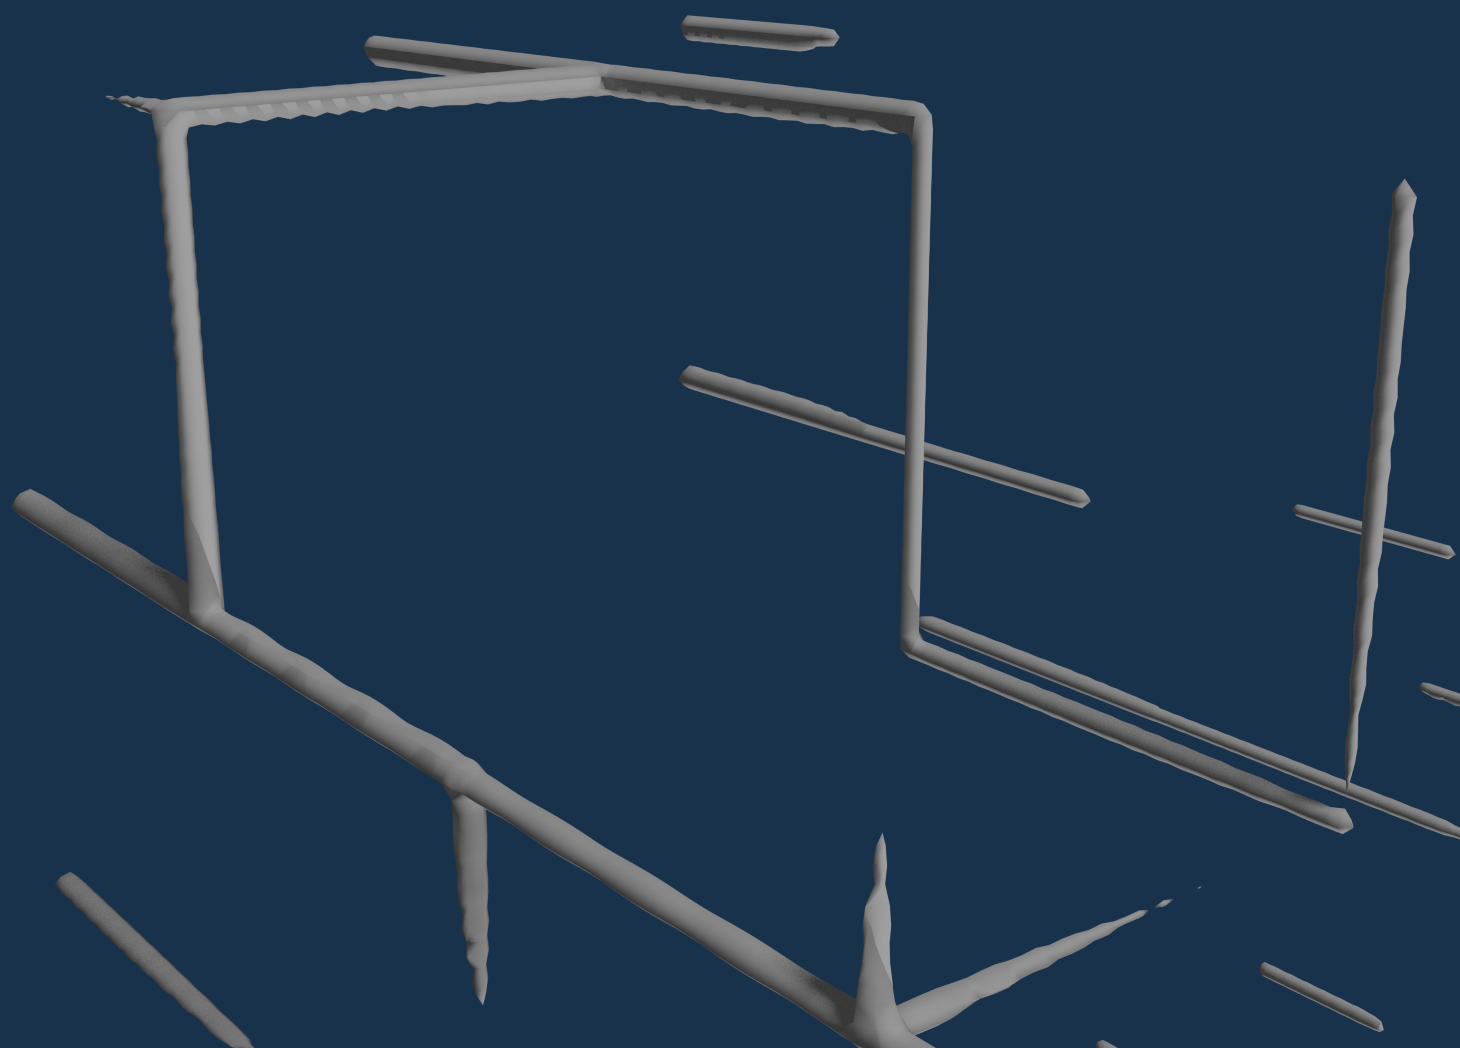
\includegraphics[width=\textwidth]{chapters/project/hiller_result.png}
  \end{center}
  \caption{Rendering of result of simulation generated by KARSTAQUIFER tool \parencite{Kaufmann200962}.
  Input data file courtesy of Mr Thomas Hiller PhD from Free University of Berlin.
  Available in file \texttt{examples\textbackslash blobber\textbackslash hiller.in}. Be advised, that
  due to very large domain, computations done by karstgen may take several hours.
  Figure rendered with Blender renderer.}
  \label{fig:hillershot}
\end{figure}

\begin{figure}[htb]
  \begin{center}
    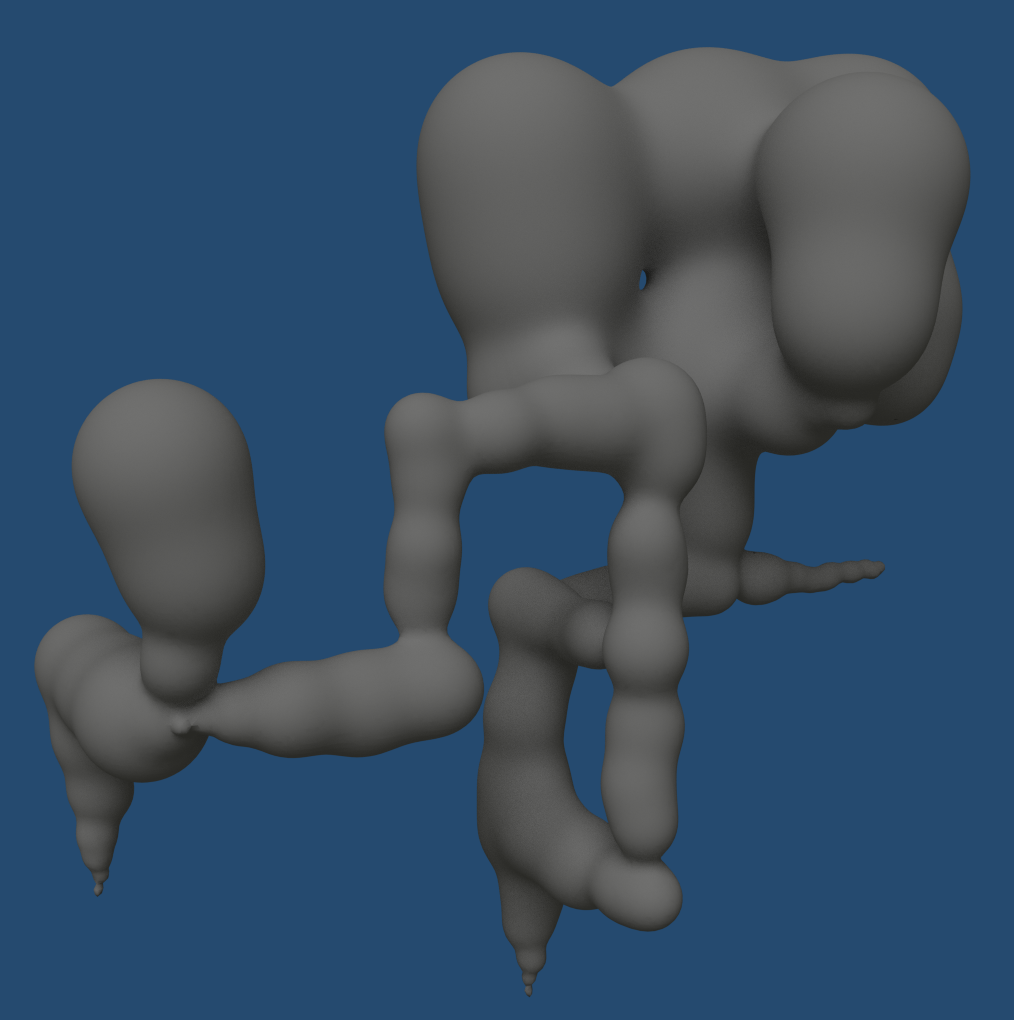
\includegraphics[width=\textwidth]{chapters/project/synthetic.png}
  \end{center}
  \caption{Render of synthetic blobber input file created by author. Rendered
    with Blender Cycles renderer. Input file available at \texttt{examples\textbackslash blobber\textbackslash synthetic.in}}
  \label{fig:synthetic}
\end{figure}

\begin{figure}[htb]
  \begin{center}
    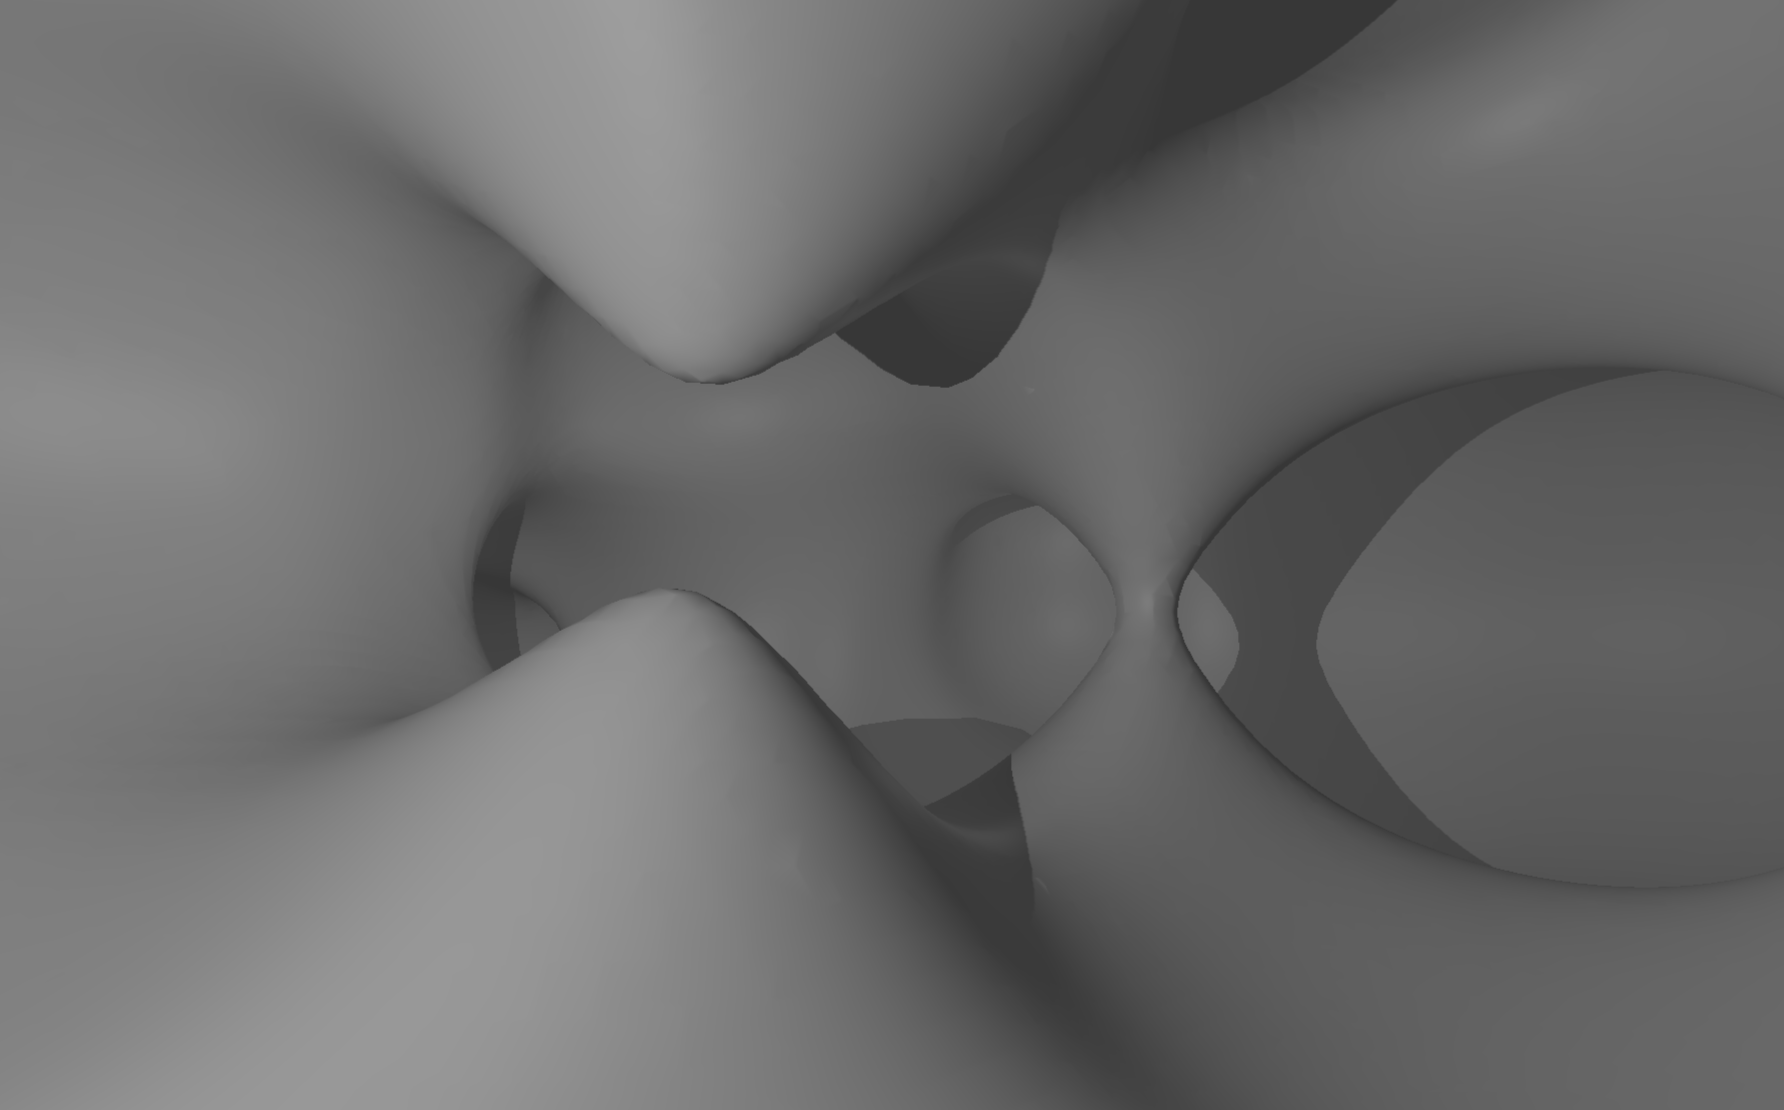
\includegraphics[width=\textwidth]{chapters/project/interior.png}
  \end{center}
  \caption{Interior of the cave generated for \autoref{fig:synthetic}. Rendered with
Blender renderer.}
  \label{fig:interior}
\end{figure}
